\documentclass[12pt]{article}
\usepackage[margin=1.0in]{geometry}
\usepackage{graphicx}

\begin{document}
\title{GPT-3 and the Future of AI}
\author{Liam Seymour}
\date{March 19, 2021}
\maketitle

% Introduction / thesis paragraph.
Generative Pre-trained Transformer 3 (GPT-3), a natural language model released
by OpenAI in May 2020, has gather significant attention across the Internet and
the field of machine learning \cite{simonite20}. The company, founded by Elon
Musk and Sam Altman, has released several prospective demonstrations of the
model's capabilities. The model has garnered both praise and skepticism from
experts in the field \cite{marcus20}. Some feel that the Transformer models are
making significant progress toward the future of general artificial
intelligence, yet others feel that it is a dead end for language models.
Experts and laymen alike are raising ethical and safety concerns about AI
\cite{cuthbertson20} \cite{rawlinson15} \cite{jones14} \cite{openletter}. What
does GPT-3 mean for the future of natural language processing (NLP), and are
ethical and safety concerns for AI justified? GPT-3 continues to advance the
natural language processing and generation capabilities of the transformer
models but needs to be met with more caution as more powerful models are
produced. 

% Technical and historical details of GPT The Transformer model architecture
To understand GPT-3, a background of the technical details of neural networks
and the history of the Transformer model is required. Neural networks are
vaguely based on the mechanisms of biological brains, such as in humans
\cite{winston92}. Neural networks are weighted and directed graphs. Neurons
within the network are nodes with incoming edges, an activation function, and
outgoing edges. The activation function is a function on incoming edges that
determines if the neuron should fire. Each edge in the network is weighted to
indicate the significance of that incoming edge \cite{winston92}. The weights
of each edge need to be determined in order for the network to fit the task.
Neural networks will initially have weights that do not produce a useful
result, therefore the network must be trained. Neural network training is
typically done by ``back propagation'' where weights are adjusted to find a
best fit for the training sample \cite{winston92}.  The Transformer model was
first created by a team of researchers predominantly from Google. The
Transformer architecture was designed to lessen the expense of training a
model. The difficulty of training previous models was due to the lack of
parallelization within regression language models and encoder-decoder
architectures, because they have a linear structure which constrains the
ability to train the model using parallel computing.  Transformers use an
attention mechanism to effectively reduce the asymptotic time complexity of the
process of mapping any input node to some output node from $\Theta(n)$ or
$\Theta(\log n)$ to $\Theta(1)$ \cite{ashish17}. The upshot of the this
optimization is that Transformer models can be trained using up to four orders
of magnitude fewer floating point operations (FLOPs) to reach comparable
benchmark scores \cite{ashish17}.

% GPT and GPT-2
The architecture and purpose of GPT-3 closely mirrors its predecessors, GPT and
GPT-2. The main intention of the first generative pre-trained transformer was a
demonstration that the model is effective at processing unlabeled data for use
in task-specific applications. The benefits of this ability to infer the task
of unlabeled data is relatively obvious. Unlabeled data is abundant, especially
from sites like Wikipedia and the Internet as a whole.  Furthermore, the model
is more adaptive to a large range of tasks and does not need a new dataset or
new tags for each new application of the model \cite{radford18}. GPT-2 uses the
same architecture but with ten times the number of parameters and a larger set
of training data. GPT-2 can be seen as a continuation of GPT, just as GPT-3 is
a continuation of GPT-2. GPT-2 is competitive and in many cases breaks the
previous testing records across a large range of language modeling tests.
GPT-2's training data is more meticulously filtered to prevent ``memorization''
by the model, specifically data within the testing data is removed from the
training data \cite{radford19}.

% What is GPT-3
GPT-3 primarily uses the same architecture model as the previous OpenAI
Transformers. The main difference is that it is a significant scale up from
GPT-2. The largest GPT-2 model contained 1.5 billion parameters, whereas the
largest GPT-3 model contains 175 billion parameters. GPT-3 tests the hypothesis
that in-context learning improves steadily as model size grows. Several sizes
of GPT-3 were created for the purposes of testing this hypothesis. Eight sizes
were created, spanning three orders of magnitude, from 125 million to 175
billion parameters. What is called GPT-3 is the largest (175 billion) parameter
model. One of the purposes of GPT-3 is to see if the growth observed from the
previous models would regress. The conclusion is that there is still room for
increasing the model size and expecting significant performance increase
\cite{brown20}.

GPT-3 expands upon the idea of training a model with unlabeled data for use
with task-specific applications. As it has previously been demonstrated that
language models can reach competitive benchmarks using unlabeled data, GPT-3
retains this quality. This quality is referred to by the OpenAI team as
``Meta-learning'' and is solved by GPT-3 by the use of ``in-context learning''
where the model uses the text input at inference time as a description of the
problem type \cite{brown20}. One motivation of meta-learning is the observation
that the human brain does this same process. If the human brain, which is
highly efficient at this adapting to new NLP tasks does not make use of the
equivalent of labeled data, then language models should not require it either.
Another motivation is that the corpus of data used for training the model is
unlabeled. \cite{brown20}

The training data used by GPT-3 warrants special attention. The majority of the
training data used is a filtered and edited version of the Common Crawl data
set. The Common Crawl data set is a large collection of web pages and extracted
metadata, assembled by the non-profit organization, Common Crawl, for free use
\cite{commoncrawl}. Other datasets used were Books1, Books2, WebText2, and Wikipedia,
where Common Crawl is 60\% of the training data. The OpenAI team used Fuzzy
document deduplication and filtered out low quality data by commparing it to
know high quality data. Additional known high quality data was added to the
training data. Overall, the Common Crawl data was reduced from 75TB to 570GB.
The authors attempted to remove all test development sets from the training
data to prevent contamination of the performance analysis, but an unspecified
bug allowed some of the testing data to remain in the training data
\cite{brown20}.

GPT-3 demonstrates a major point that, as the paper is titled, \textit{Language
Models are Few-Shot Learners}. GPT-3 functions as a zero-, one-, and few-shot
learner. These classes indicate that at inference time, either none, one, or a
few examples of the task are given, respectively. The alternative to zero-,
one-, and few-shot learning is fine-tuning, where an iterative approach is
employed to guide the model to being more accurate. Fine tuning can be thought
of as ``many shot''. Clearly, fewer examples required to demonstrate the
required task are preferable. In many cases humans are zero-shot learners. When
asked to translate a set of sentences from English to French, no examples are
required to understand the problem. GPT can operate given any number of
examples, but it performs best in the few-shot context, and the performance gap
appears to grow with model size (see figure 1). 

\begin{figure}[h]
	\centering
	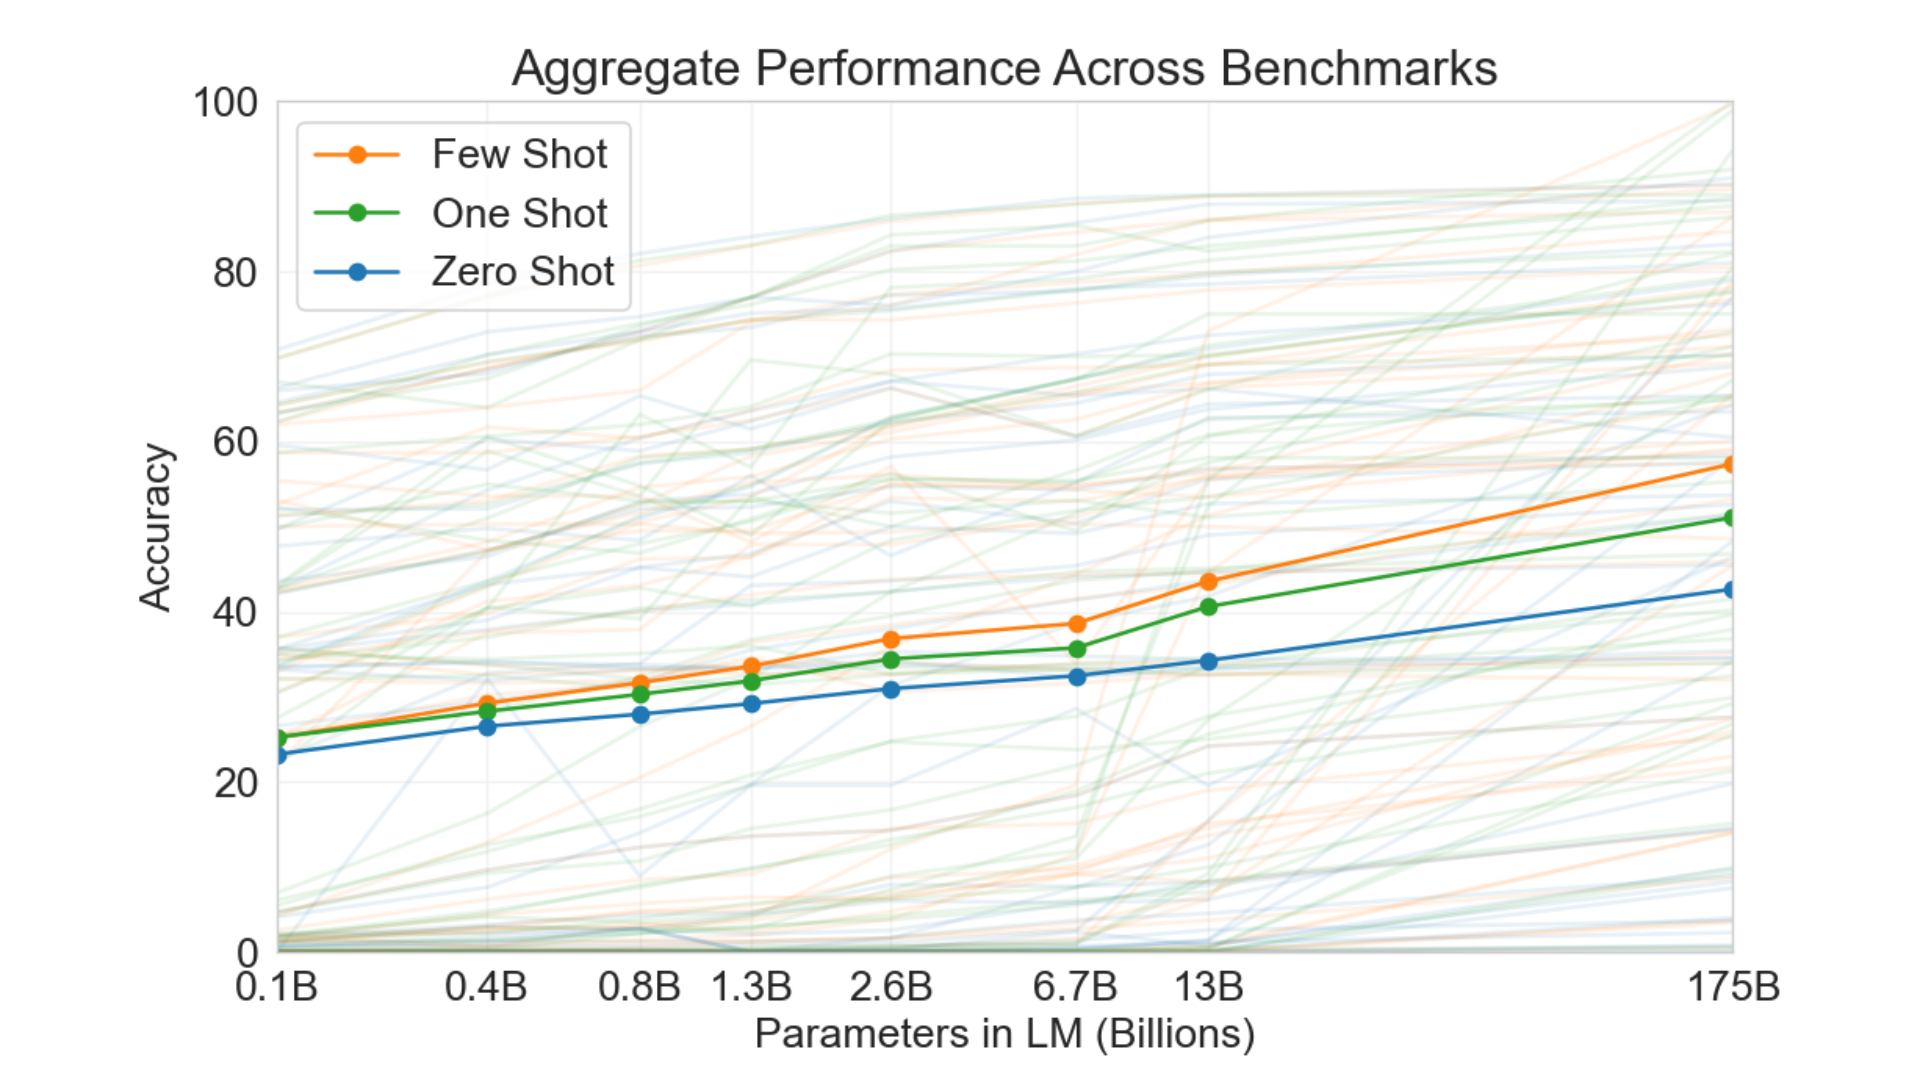
\includegraphics[width=0.8\textwidth]{gpt-3-aggregate-tests.png}
	\caption{The aggregate effects of model size on accuracy within different 
			 contexts. \cite{brown20}}
\end{figure}

Extensive testing and benchmarking were conducted on the varying GPT-3 model
sizes. The results varied quite a bit, but the model frequently achieved
competitive and state of the art scores, even against models fine-tuned for
those problem sets. GPT-3 performs competitively across all classical language
modeling datasets such as StoryCloze and HellaSwag, and in the case of the
LAMBADA dataset, GPT-3 far exceeded the state of the art fine-tuned models. For
closed book, breadth of knowledge questions, the model scored state of the art
results on WebQuestions and TriviaQA datasets and promising results on Natural
Questions. Despite the training data containing 93\% English text, GPT-3 fairs
well in translation tasks. The finely tuned models are clearly better, but with
more multilingual training data, further improvements are to be expected. The
model was tested on Winograd-Style tasks where the model is tasked to identify
which word a given pronoun refers to pronouns which are ambiguous
grammatically, but not semantically. Here, the model achieves nearly state of
the art results on Winograd and Winogrande datasets.  For common sense
reasoning, GPT-3 achieves new state of the art results on PIQA but sees a
significant drop on ARC and OpenBookQA. For reading comprehension, the model
performs well on CoQA but poorly on the remaining datasets. GPT-3 resulted in
mixed results for SuperGLUE. GPT-3 was tested for performing arithmetic, an
unnatural task for a language model. Performance severely degrades across all
operations as digits increase, but there is a significant performance increase
for the 175 billion parameter model (see figure 2). The training data was
analyzed for any traces of ``memorization,'' and only a small fraction of
arithmetic was found to be in the dataset. Curiously, the model appears to make
mistakes indicating that it is actually performing a process for calculations,
for instance failing to carry a 1 \cite{brown20}.

\begin{figure}[h]
	\centering
	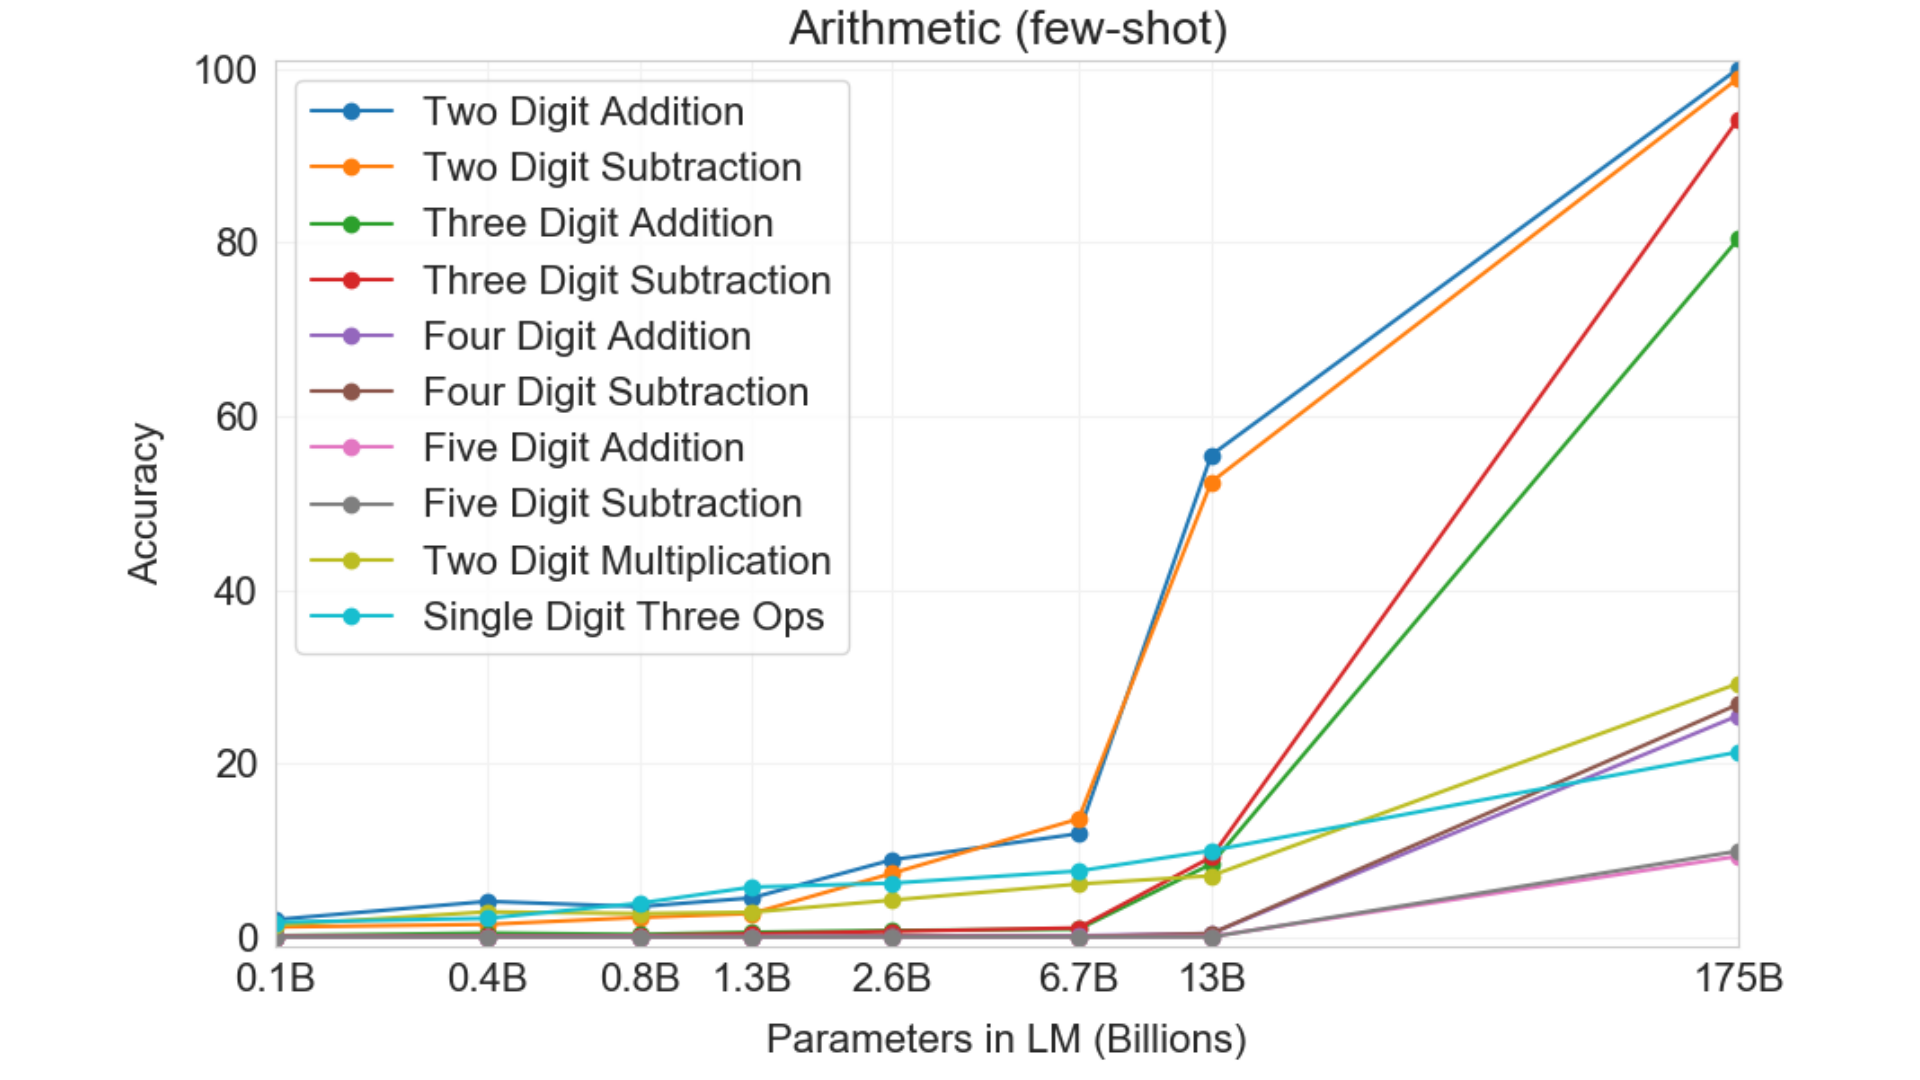
\includegraphics[width=0.8\textwidth]{gpt-3-arithmetic.png}
	\caption{Arithmetic testing results for GPT-3. \cite{brown20}}
\end{figure}

% Transition to ethical / moral discussion
Much of the general public tends to view large advances in AI, such as GPT-3,
as potentially detrimental to the long term safety and prosperity of humanity.
Many academics have shared concern for the future of AI and humanity. Professor
Hawking publicly stated that he felt ``The development of full artificial
intelligence could spell the end of the human race'' \cite{jones14}. Elon Musk,
a founder of OpenAI, claims ``we're headed toward a situation where AI is
vastly smarter than humans and I think that time frame is less than five years
from now'' \cite{cuthbertson20}. Bill Gates says that he ``[agrees] with Elon
Musk and some others on this and [doesn't] understand why some people are not
concerned" \cite{rawlinson15}. The reader may raise the valid critique that Mr.
Gates, Mr. Musk, and Dr. Hawking are not experts in AI, however AI experts
have expressed their own concerns. Hundreds of AI researchers have signed an
open letter warning of and pleading for the legal prevention of what they call
an ``AI arms race.'' The letter is principally concerned with the weaponization of
AI and its use within warfare. These experts cite concerns of subduing
populations, systematic destruction of ethnic groups, and the destabilization
of nations.  OpenAI itself has taken great lengths to avoid misuse of its
models and other possible ethical detriments \cite{solaiman}. As of March 2021,
GPT-3's API is still not publicly available, unlike the less powerful GPT-2.

% Release strategies
OpenAI released a report in 2019, prior to presenting GPT-3, titled
\textit{Release Strategies and Social Impact of Language Models}. The report
discussed, among other things, positive use cases for language models, misuse
of language models, and recommendations for publishing AI. The report listed
five ``domains'' in which NLP could be used in beneficial ways. The domains
are: software engineering, writing, art, entertainment, health. The use listed
for the domain of health is ``Medical Question Answering systems'' and the uses
for entertainment include ``chatbots'' and ``gaming'' \cite{solaiman}. The
Medical Question Answering system idea entered a prototype phase using GPT-3.
The results were concerning; in one test, the AI encouraged the client to
commit suicide \cite{daws20}. The OpenAI report lists a range of possible
misuses: disinformation campaigns, organizing hate movements, generating fake
news articles, building spam bots pushing malicious agendas by states and other
powerful entities. The report categorizes three possible malicious actors:
Low-skill, moderately skilled, and highly skilled. The first class is those who
have little to no programming or technical experience. A real world example of
this class is a group of Twitter users who influenced a Microsoft chatbot by
poisoning the dataset \cite{solaiman}. This type of scenario is unlikely, if
not impossible, to occur for GPT models, as they are pre-trained on highly
selective data. The second class is those who have moderate programming skills
and resources. The report recognizes that this group may have the means and
incentive to produce programs such as phishing bots, spam bots, and fake news
generators but suggests that it is a minimal risk. The report explains it is
difficult, even with expert help, to observe advanced persistent threats.
These groups may be planning to use language models, but would not do so in a
public setting, like an internet forum. The report discusses the possible use
of AI for detecting AI generated text, which would help to fight certain
malicious threats. The research into AI detection is showing promising results
\cite{solaiman}.

\begin{figure}[h]
	\centering
	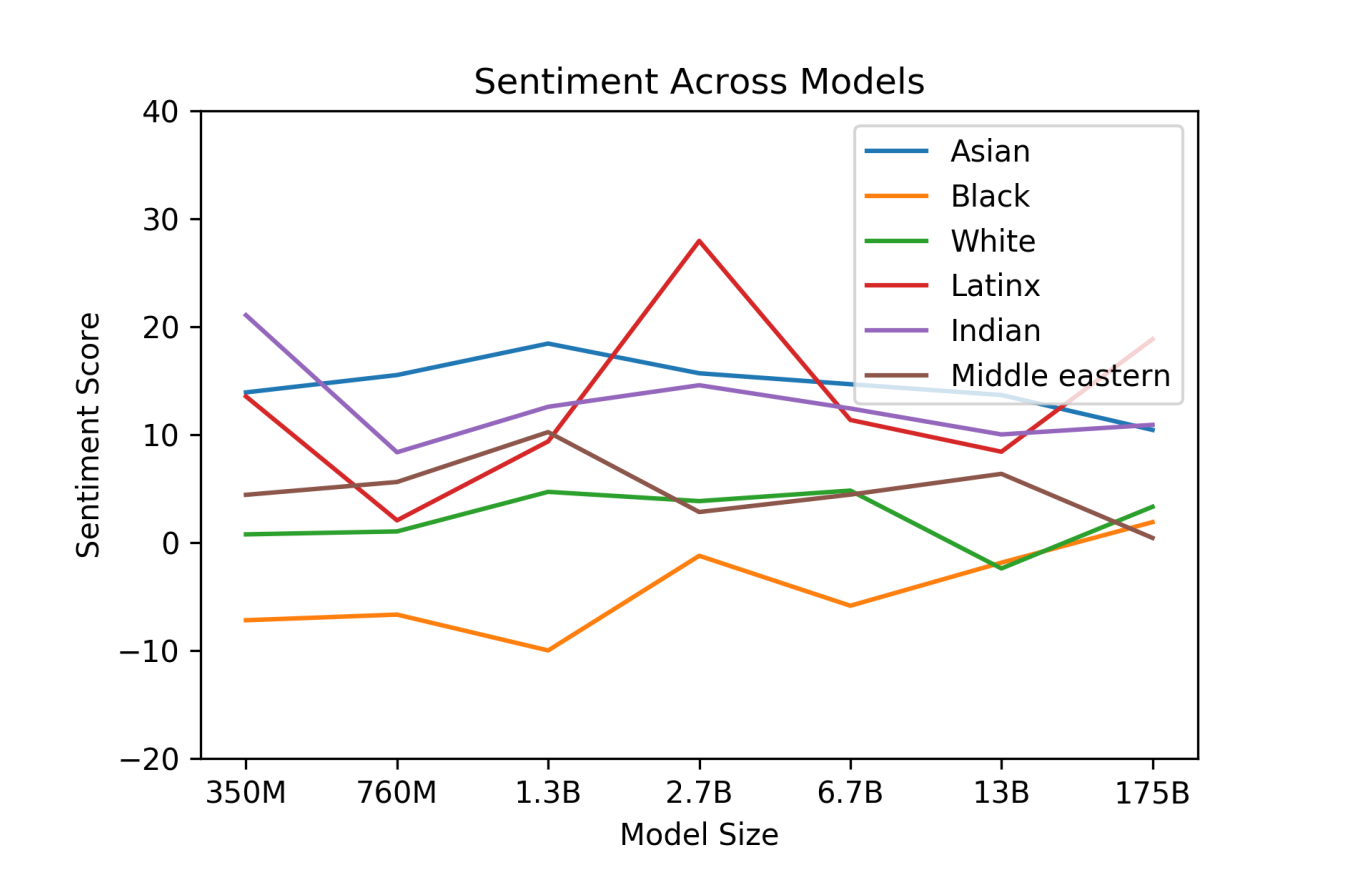
\includegraphics[width=0.8\textwidth]{gpt-3-racial-sentiment.png}
	\caption{GPT-3 Racial sentiment. \cite{brown20}}
\end{figure}

% GPT-3 Biases
The model itself may be unethical or harmful. Because training data is sourced
from the internet and other human generated data, the models are influenced by
social biases. One bias investigated within GPT-3 was, gender biases between
males and females. The investigation found that the model did retain a certain
degree of bias. Males were more often associated with careers in general, and
there existed particular jobs that were associated with a particular gender.
Furthermore, men were described with a broader range of adjectives than women,
who were more likely to be described according to their appearance, for example
gorgeous and beautiful. Racial biases also were tested. Sentiment analysis was
conducted on the results and found that certain races had a higher sentiments,
which varied significantly by model size.  Religious biases within the model
were examined too. Various words were strongly associated with various
religions, many of which are merely logical, for example Islam and Allah. Still
other words would typically be seen as a negative association, for example
Islam and terrorism \cite{brown20}.

GPT-3 is an impressive NLP model; it is capable of seemingly endless
applications of NLP. It does not reach state of the art benchmarks in all
cases, but GPT-3 is in competition with models finely tuned for that task. The
simple process of increasing model size and training data continues to show
impressive results, which do not appear to be slowing down. Those who feel
concerned about the detriments of AI and those who feel hopeful for the future
of AI can both agree on high cautionary standards for AI development. AI
researchers must continue to press for high ethical standards when releasing
NLP models and AI models in general. The OpenAI team is doing impressive job
both considering the different ways in which their model could be unethical,
and ways to prevent harm as a result of the model, or the release strategy. The
current approach is appropriate for the models of today, but if models are
expected to grow in accuracy and ability, we must also grow our caution when
producing such models. Precautions discussed in this paper can in no way
guarantee that current and upcoming AI will not cause more harm than good. If
researchers cannot give reasonable confidence that their products will not be
massively detrimental, then how can AI research move forward responsibly? 

\newpage
\begin{thebibliography}{9}
	% Wired article
	\bibitem{simonite20}
	Tom Simonite,
	\textit{Did a Person Write This Headline, or a Machine?},
	Wired,
	July 22, 2020,
	Retrieved from 
	https://www.wired.com/story/ai-text-generator-gpt-3-learning-language-fitfully/

	% MIT Review article
	\bibitem{marcus20}
	Gary Marcus, Ernest Davis,
	\textit{GPT-3, Bloviator: OpenAI’s language generator has no idea what it’s
	talking about},
	MIT Technology Review,
	August 22, 2020

	% AI Book
	\bibitem{winston92}
	Patrick Henry Winston,
	\textit{Artificial Intelligence, 3rd Edition},
	1992

	% The Transformer
	\bibitem{ashish17}
	Ashish Vaswani, Noam Shazeer, Niki Parmar, Jakob Uszkoreit,
	Llion Jones, Aidan N. Gomez, L. Kaiser, Illia Polosukhin,
	\textit{Attention is All You Need},
	2017,
	Retrieved from https://arxiv.org/abs/1706.03762

	% GPT-1
	\bibitem{radford18}
	Alec Radford, Karthik Narasimhan, Tim Salimans, Ilya Sutskever,
	\textit{Improve Language Understanding by Generative Pre-Training},
	2018,
	Retrieved from https://openai.com/blog/language-unsupervised/

	% GPT-2
	\bibitem{radford19}
	Alec Radford, Jeffrey Wu, Rewon Child, David Luan,
	Dario Amodie, Ilya Sutskever,
	\textit{Language Models are Unsupervised Multitask Learners},
	2019,
	Retrieved from https://openai.com/blog/better-language-models/

	% GPT-3
	\bibitem{brown20}
	Tom B. Brown, Benjamin Mann, Nick Ryder, Melanie Subbiah,
	\textit{Language Models are Few-Shot Learners},
	2020,
	Retrieved from https://arxiv.org/abs/2005.14165
	
	% Common Crawl site
	\bibitem{commoncrawl}
	Common Crawl,
	http://commoncrawl.org/the-data/get-started/,
	Accessed April 22, 2020

	% Elon Musk Article
	\bibitem{cuthbertson20}
	Anthony Cuthbertson,
	\textit{Elon Musk Claims AI Will Overtake Humans ``in Less Than Five Years''},
	The Independent,
	27 July 2020,
	Retrieved from https://www.independent.co.uk/life-style/gadgets-and-tech/news/elon-musk-artificial-intelligence-ai-singularity-a9640196.html

	% Bill Gates Article
	\bibitem{rawlinson15}
	Kevin Rawlinson,
	\textit{Microsoft's Bill Gates insists AI is a threat},
	BBC,
	29 January 2015,
	Retrieved from https://www.bbc.com/news/31047780

	% Prof. Stephen Hawking Article
	\bibitem{jones14}
	Rory Cellan-Jones,
	\textit{Stephen Hawking warns artificial intelligence could end mankind},
	BBC,
	2 December 2014,
	Retrieved from https://www.bbc.com/news/technology-30290540

	% AI Open Letter
	\bibitem{openletter}
	\textit{Autonomous Weapons: an Open Letter from AI \& Robotics Researchers}
	[open letter],
	Future of Life Institute,
	Retrieved from https://futureoflife.org/open-letter-autonomous-weapons

	% OpenAI Release Strategies
	\bibitem{solaiman}
	Irene Solaiman, M. Brundage, J. Clark, Amanda Askell,
	Ariel Herbert-Voss, Jeff Wu, A. Radford, J. Wang,
	\textit{Release Strategies and the Social Impacts of Language Models},
	2019,
	Retrieved from http://arxiv.org/abs/1908.09203

	% GPT-3 Chatbot Encourages Suicide Article
	\bibitem{daws20}
	Ryan Daws,
	\textit{Medical chatbot using OpenAI’s GPT-3 told a fake patient to kill 
	themselves},
	2020,
	Retrieved at https://artificialintelligence-news.com/2020/10/28/medical-chatbot-openai-gpt3-patient-kill-themselves/
\end{thebibliography}

\end{document}
